% !Mode:: "TeX:UTF-8"
%# -*- coding:utf-8 -*-

%% 使用 njuthesis 文档类生成南京大学学位论文的示例文档
%%作者:njuhan: https://github.com/njuHan
%% 部分提纲取自njuhan的本科毕业论文

\documentclass[winfonts,master,oneside,nobackinfo]{njuthesis}
%% njuthesis 文档类的可选参数有:
%%   nobackinfo 取消封二页导师签名信息。注意,按照南大的规定,是需要签名页的。
%%   phd/master/bachelor 选择博士/硕士/学士论文

\usepackage{lipsum}
\usepackage{listings}
\usepackage{xcolor}
\lstset{breaklines}%这条命令可以让LaTeX自动将长的代码行换行排版
\lstset{extendedchars=false}%这一条命令可以解决代码跨页时,章节标题,页眉等汉字不显示的问题
\lstset{                        %Settings for listings package.
  language=[ANSI]{C},
  backgroundcolor=\color{white},
  basicstyle=\footnotesize,
  breakatwhitespace=false,
  breaklines=true,
  captionpos=b,
  commentstyle=\color{olive},
  directivestyle=\color{blue},
  extendedchars=false,
  % frame=single,%shadowbox
  framerule=0pt,
  keywordstyle=\color{blue}\bfseries,
  morekeywords={*,define,*,include...},
  numbersep=5pt,
  rulesepcolor=\color{red!20!green!20!blue!20},
  showspaces=false,
  showstringspaces=false,
  showtabs=false,
  stepnumber=2,
  stringstyle=\color{purple},
  tabsize=4,
  title=\lstname
}


%%%%%%%%%%%%%%%%%%%%%%%%%%%%%%%%%%%%%%%%%%%%%%%%%%%%%%%%%%%%%%%%%%%%%%%%%%%%%%%
% 设置《国家图书馆封面》的内容,仅博士论文才需要填写

% 设置论文按照《中国图书资料分类法》的分类编号
\classification{0175.2}
% 论文的密级。需按照GB/T 7156-2003标准进行设置。预定义的值包括:
% - \openlevel,表示公开级:此级别的文献可在国内外发行和交换。
% - \controllevel,表示限制级:此级别的文献内容不涉及国家秘密,但在一定时间内
%   限制其交流和使用范围。
% - \confidentiallevel,表示秘密级:此级别的文献内容涉及一般国家秘密。
% - \clasifiedlevel,表示机密级:此级别的文献内容涉及重要的国家秘密 。
% - \mostconfidentiallevel,表示绝密级:此级别的文献内容涉及最重要的国家秘密。
% 此属性可选,默认为\openlevel,即公开级。
\securitylevel{\controllevel}
% 设置论文按照《国际十进分类法UDC》的分类编号
% 该编号可在下述网址查询:http://www.udcc.org/udcsummary/php/index.php?lang=chi
\udc{004.72}
% 国家图书馆封面上的论文标题第一行,不可换行。此属性可选,默认值为通过\title设置的标题。
\nlctitlea{数据中心}
% 国家图书馆封面上的论文标题第二行,不可换行。此属性可选,默认值为空白。
\nlctitleb{网络模型研究}
% 国家图书馆封面上的论文标题第三行,不可换行。此属性可选,默认值为空白。
\nlctitlec{}
% 导师的单位名称及地址
\supervisorinfo{南京大学计算机科学与技术系~~南京市汉口路22号~~210093}
% 答辩委员会主席
\chairman{张三丰~~教授}
% 第一位评阅人
\reviewera{阳顶天~~教授}
% 第二位评阅人
\reviewerb{张无忌~~副教授}
% 第三位评阅人
\reviewerc{黄裳~~教授}
% 第四位评阅人
\reviewerd{郭靖~~研究员}


%%%%%%%%%%%%%%%%%%%%%%%%%%%%%%%%%%%%%%%%%%%%%%%%%%%%%%%%%%%%%%%%%%%%%%%%%%%%%%%
% 设置论文的中文封面

% 论文标题,不可换行
\title{南大本科毕业论文\LaTeX 模板}
% 如果论文标题过长,可以分两行,第一行用\titlea{}定义,第二行用\titleb{}定义,将上面的\title{}注释掉
% \titlea{半轻衰变$D^+\to \omega(\phi)e^+\nu_e$的研究}
% \titleb{和弱衰变$J/\psi \to D_s^{(*)-}e^+\nu_e$的寻找}

% 论文作者姓名
\author{作者}
% 论文作者联系电话
\telphone{xxxx}
% 论文作者电子邮件地址
\email{sample@smail.nju.edu.cn}
% 论文作者学生证号
\studentnum{12xxxxxxx}
% 论文作者入学年份(年级)
\grade{2012}
% 导师姓名职称
\supervisor{某~~教授}
% 导师的联系电话
\supervisortelphone{}
% 论文作者的学科与专业方向
\major{计算机科学与技术}
% 论文作者的研究方向
\researchfield{分布式计算}
% 论文作者所在院系的中文名称
\department{计算机科学与技术系}
% 论文作者所在学校或机构的名称。此属性可选,默认值为``南京大学''。
\institute{南京大学}
% 论文的提交日期,需设置年、月、日。
\submitdate{2016年\qquad 月\qquad 日}
% 论文的答辩日期,需设置年、月、日。
\defenddate{2016年\qquad 月\qquad 日}
% 论文的定稿日期,需设置年、月、日。此属性可选,默认值为最后一次编译时的日期,精确到日。
\date{2016年6月8日}

%%%%%%%%%%%%%%%%%%%%%%%%%%%%%%%%%%%%%%%%%%%%%%%%%%%%%%%%%%%%%%%%%%%%%%%%%%%%%%%
% 设置论文的英文封面

% 论文的英文标题,不可换行
\englishtitle{\LaTeX \;  NJU thesis template }
% 论文作者姓名的拼音
\englishauthor{Author}
% 导师姓名职称的英文
\englishsupervisor{ Professor}
% 论文作者学科与专业的英文名
\englishmajor{Computer Science and Technology}
% 论文作者所在院系的英文名称
\englishdepartment{Department of Computer Science and Technology}
% 论文作者所在学校或机构的英文名称。此属性可选,默认值为``Nanjing University''。
\englishinstitute{Nanjing University}
% 论文完成日期的英文形式,它将出现在英文封面下方。需设置年、月、日。日期格式使用美国的日期
% 格式,即``Month day, year'',其中``Month''为月份的英文名全称,首字母大写;``day''为
% 该月中日期的阿拉伯数字表示;``year''为年份的四位阿拉伯数字表示。此属性可选,默认值为最后
% 一次编译时的日期。
\englishdate{May 20th, 2016}

%%%%%%%%%%%%%%%%%%%%%%%%%%%%%%%%%%%%%%%%%%%%%%%%%%%%%%%%%%%%%%%%%%%%%%%%%%%%%%%
% 设置论文的中文摘要

% 设置中文摘要页面的论文标题及副标题的第一行。
% 此属性可选,其默认值为使用|\title|命令所设置的论文标题
% \abstracttitlea{数据中心网络模型研究}
% 设置中文摘要页面的论文标题及副标题的第二行。
% 此属性可选,其默认值为空白
% \abstracttitleb{}

%%%%%%%%%%%%%%%%%%%%%%%%%%%%%%%%%%%%%%%%%%%%%%%%%%%%%%%%%%%%%%%%%%%%%%%%%%%%%%%
% 设置论文的英文摘要

% 设置英文摘要页面的论文标题及副标题的第一行。
% 此属性可选,其默认值为使用|\englishtitle|命令所设置的论文标题
\englishabstracttitlea{englishabstracttitlea}
% 设置英文摘要页面的论文标题及副标题的第二行。
% 此属性可选,其默认值为空白
\englishabstracttitleb{nglishabstracttitleb}

%%%%%%%%%%%%%%%%%%%%%%%%%%%%%%%%%%%%%%%%%%%%%%%%%%%%%%%%%%%%%%%%%%%%%%%%%%%%%%%
\begin{document}

%%%%%%%%%%%%%%%%%%%%%%%%%%%%%%%%%%%%%%%%%%%%%%%%%%%%%%%%%%%%%%%%%%%%%%%%%%%%%%%

% 制作国家图书馆封面(博士学位论文才需要)
%\makenlctitle
% 制作中文封面
\maketitle
% 制作英文封面
\makeenglishtitle


%%%%%%%%%%%%%%%%%%%%%%%%%%%%%%%%%%%%%%%%%%%%%%%%%%%%%%%%%%%%%%%%%%%%%%%%%%%%%%%
% 开始前言部分
\frontmatter

%%%%%%%%%%%%%%%%%%%%%%%%%%%%%%%%%%%%%%%%%%%%%%%%%%%%%%%%%%%%%%%%%%%%%%%%%%%%%%%
% 论文的中文摘要
\begin{abstract}
\lipsum[1-2]

%通过改变链路中子流的个数,分配不同的数据流量给不同的链路。

% 中文关键词。关键词之间用中文全角分号隔开,末尾无标点符号。
\keywords{关键词1 \quad 关键词2 }
\end{abstract}

%%%%%%%%%%%%%%%%%%%%%%%%%%%%%%%%%%%%%%%%%%%%%%%%%%%%%%%%%%%%%%%%%%%%%%%%%%%%%%%
% 论文的英文摘要
\begin{englishabstract}
\lipsum[2]

%Rate adaptation can be implemented by adjusting the number of subflows on each path.

% 英文关键词。关键词之间用英文半角逗号隔开,末尾无符号。
\englishkeywords{keyword1\quad keyword2}
\end{englishabstract}

%%%%%%%%%%%%%%%%%%%%%%%%%%%%%%%%%%%%%%%%%%%%%%%%%%%%%%%%%%%%%%%%%%%%%%%%%%%%%%%
% 论文的前言,应放在目录之前,中英文摘要之后
%
\begin{preface}
\lipsum[1]
\vspace{1cm}
\begin{flushright}
作者\\
20xx年夏于南京大学
\end{flushright}

\end{preface}

%%%%%%%%%%%%%%%%%%%%%%%%%%%%%%%%%%%%%%%%%%%%%%%%%%%%%%%%%%%%%%%%%%%%%%%%%%%%%%%
% 生成论文目录
\tableofcontents

%%%%%%%%%%%%%%%%%%%%%%%%%%%%%%%%%%%%%%%%%%%%%%%%%%%%%%%%%%%%%%%%%%%%%%%%%%%%%%%
% 生成插图清单。如无需插图清单则可注释掉下述语句。
\listoffigures

%%%%%%%%%%%%%%%%%%%%%%%%%%%%%%%%%%%%%%%%%%%%%%%%%%%%%%%%%%%%%%%%%%%%%%%%%%%%%%%
% 生成附表清单。如无需附表清单则可注释掉下述语句。
\listoftables

%%%%%%%%%%%%%%%%%%%%%%%%%%%%%%%%%%%%%%%%%%%%%%%%%%%%%%%%%%%%%%%%%%%%%%%%%%%%%%%
% 开始正文部分
\mainmatter

%%%%%%%%%%%%%%%%%%%%%%%%%%%%%%%%%%%%%%%%%%%%%%%%%%%%%%%%%%%%%%%%%%%%%%%%%%%%%%%
% 学位论文的正文应以《绪论》作为第一章
\chapter{绪论}\label{chapter_introduction}
\section{研究背景及意义}
互联网自诞生于上个世纪以来,正一步一步的改变这地球上每个人的生活。特别是伴随移动通信技术的革新,结合互联网技术和移动通信技术的移动互联网正深刻地改变着生活的方方面面。饮食、购物、交通、居住、社交、娱乐等等方面,在当下的移动互联时代都有了新的运作生态。随着移动互联技术的成熟和在“摩尔定律”下硬件成本的降低,人们越来越容易地融入互联网时代,根据中国互联网络信息中心发布的数据,截至2018年6月,我国网民规模已经超过了8亿,渗透率近六成,而其中移动互联网用户比例高达98\%。海量的用户在使用互联网时也正有意无意地创造着海量的数据,而海量的数据中蕴藏着巨大的价值。这些数据的类型包括数值型数据、文本型数据、图片型数据、视频型数据、音频型数据等,利用好这些不同类型的数据可以创造出大量的经济价值和社会价值。

自然语言处理技术(Natural language processing)是计算机信息工程的一个子领域,目标便是处理和分析海量的文本数据,使得计算机程序可以利用词法、语法、语义等信息对自然语言文本完成识别、理解与输出等任务,例如词语分割、命名实体识别、关系抽取、机器翻译、自然语言生成、问答系统、情感分析等等。自然语言技术通过规则学习、统计学习等方法的研究与探索日臻成熟。近十年,表示学习、深度神经网络类机器学习技术给自然语言处理技术带来了新的探索与发展,在部分自然语言处理问题上可以达到良好而稳定的结果。自然语言处理技术在各行各业有着多种应用:社交媒体上的评论文本数据可以用来辅助监测舆情舆论的走向;财经新闻中包含诸多经济数据、公司运营情况,利用这些文本数据可以辅助量化交易的执行;利用新闻媒体中的海量文本数据,我们可以对用户兴趣话题进行建模,高效地为读者进行内容过滤和兴趣推荐;机器翻译技术可以将不同语言为载体的文献自动翻译,促进不同文化间的沟通和交流;知识图谱技术可以链接不同的人和组织,构造知识库,服务与多种商业应用。

命名实体识别(Named-entity recognition),又称实体抽取技术、实体分块技术,是自然语言处理技术的一个子问题。目标在于将非结构化文本中提及的命名实体抽取出来,例如人名,组织名,地点名,医疗术语法规术语,时间,数量,货币价值等等。例如在财经文章中需要准确地抽取企业名称、重要人物名称、货币价值等命名实体;在政治新闻中需要准确地抽取政治人物名称、国家地理名称、组织机构名称、事件名称等命名实体;在判决文书文本中,需要抽取出当事人名称、处罚条款、量刑情况、关联组织等信息。可以说,命名实体识别问题是自然语言处理最基础的任务之一,命名实体识别的准确率、召回率的高低直接影响着后续自然语言处理问题,例如信息抽取、文本分类、文本摘要、问答系统等等研究方向。

因而研究中文命名实体识别问题,对于中文自然语言处理技术的研究有着关键性的地位。通用命名实体技术对于中文命名实体识别有着不错的效果,然而中文与其他许多种语言的构词、语法有着诸多不同。特别是词语的边界模糊、无大小写和时态词型的变化、一词多性,一字多义、简称方法独特等等独特之处,因而相适应地根据中文语言的特点对通用命名实体技术进行优化有着很强的必要性。因而针对中文语言的各种特点,相适应地研究如何提高命名实体识别的效果就有着重要的意义。



\section{国内外研究现状}
\subsection{命名实体识别问题的定义}
命名实体识在信息抽取和自然语言处理工作中有着重要的地位。例如在一段文本中准确地识别人名、地名、组织名、时空表达等等要素,对后续其他的自然语言处理过程有着基石作用。人们对该问题的研究历程中使用过很多很多种方法,大体上这些方法可以分为知识工程方法和机器学习方法。一个典型的命名实体识别系统的输入应该是输入的自然语言文本,而输出应该是抽取出的信息并包括这些信息的边界,以及这些信息分别属于什么样的命名实体类型。例如“小明在小雨的陪同下,一起在南京看了中国国家队的比赛。”这样的一个文本输入,命名实体识别系统应该给出,“小明”、“小雨”【人物】,“南京”【地点】,“中国国家队”【组织名】这样的输出。

命名实体识别研究是一个较宽泛的范围,影响命名实体识别工作方法方案的有以下几个因素\cite{ASTUDY}:

(1)语言因素。目前,大量的研究工作都是以英文为研究对象,但是这些方案并不一定可以推广到所有的语言。例如几个东方文明的语言中文日文韩文语并不像英文单词那样有着天然的空格作为隔断,而且也不存在字母的大小写,这些特性都会使得命名实体识别的方法上有着较大的差异。就算是同是西语概念下的法文德文西班牙文等也有自身语言的特殊性。除英文外目前中文日文法文意大利文希腊文已经有了大量研究,收集整理了大量的语料和工具。针对印度文丹麦文韩文土耳其文等语言的研究也在一直的进步中。这些工作很多都是限定在自己的语言边界内,研究出一个跨语言跨文化的命名实体识别模型是当下的一个目标。

(2)领域因素。最初命名实体识别的很多工作是面对半结构化的数据,例如病历、报名表、简历、申请材料这样的文本,这些工作有各自不同的特殊性方法中会使用很多先验知识,因而技术技巧的移植困难。除此之外,文本所属领域的不同对命名实体识别工作影响也很大,文本内容属于科学技术文章或是商业、体育、旅游等领域,这些不同的领域内容也会对最终命名实体识别的效果产生很大的影响。因此,最终一个效果良好稳定可靠的命名实体识别系统需要拥有尽可能多的不同领域的预料,找到并实时更新大量不同领域的语料库也是目前一个相当大的挑战。

(3)实体和标注方法。命名实体这样一个概念在不同的语境和不同的业务需求下是有区别的。大多数的命名实体识别的研究将实体的类别分为“人”、“地点”、“组织”三类。这种分类方法 在MUC-6(6th Message Understanding Conference,命名实体识别重要会议)中被确定为一个标准称为“Enamex”分类法。然而许多文章指出这种分类方法较为粗糙,类别还可以继续细分,比如“人”这个标签下可以分为“医生”、“政治人物”、“艺人”等等,“地点”也可以为分为“国家”、“州省”、“景区”等等。

\subsection{传统方法研究发展现状}
早期命名实体识别任务并不统一,主要目标是要从一堆文本数据中自动识别出命名实体。最早的相关研究论文是1991年Rau\cite{Rau}在人工智能应用会议上发表的,论文介绍了一个自动识别公司名称的系统。主要的方法是采用启发式方法和手工规则。1996年,命名实体识别这个术语在MUC-6会议上被R. Grishman和Sundheim正式提出,该领域被越来越多的人关注,进入快速发展时期。

然而早期的研究大多还是主要依靠手工规则等办法,后来用有监督的机器学习方法逐渐火热起来。规则的设计大多是基于特殊的领域知识。Kim\cite{Kim}用规则的的方法对于口语输入的文本进行自动的命名实体识别。在生物医学领域,Hanisch\cite{Hanisch}利用预处理的同义词点来识别生物医学文本中提到的潜在的蛋白质术语。Quimbaya\cite{Quimbaya}等提出了一个基于词典的方法来提取电子医疗记录中的命名实体。实验结果表明这样的方法在提高召回率上很有效,但是在提高准确率上效果有限。大多数这样基于手工规则的方法都是利用启发式的语法语义特点,或是要用到领域内特殊的知识做成字典。这些系统在提高识别的精确的和召回度上都有很多局限。

很多学者在命名实体识别任务中引入了基于特征的有监督统计学习方法。命名实体识别问题被建模为一个多分类的任务或者一个序列标注任务。将有标注的样例数据交给模型训练,利用机器学习算法来识别其他数据中潜在的类似的命名实体模式。在这一类方法中,特征工程就会起到关键作用。单词的表示方法\cite{Nadeau},单词的的特征(如形态、读音等)\cite{Settles}、文本语料的特征(局部句法特征和出现次数等)\cite{Ravin}等等自然语言固有的特性都被用来提高识别的效果。不同的机器学习模型也会带来不同的识别效果。经典的有监督机器学习模型被一一引入命名实体识别系统:隐马尔科夫模型(HMM)\cite{Eddy}、决策树模型(DT)\cite{Quinlan}、最大熵模型(ME)\cite{Kapur}、支持向量机模型(SVM)\cite{Hearst},条件随机场模型(CRF)\cite{Lafferty}。这些有监督机器学习模型读入大量带标签的训练语料,学习出命名实体的特征,最终对新的语料中的命名实体进行预测。

针对标注训练语料费时费力,而大量未标注的数据容易获得的情况,半监督学习方法在许多学者的尝试下引入了命名实体识别问题。S. Brin\cite{Brin}利用词汇的特征,通过半监督学习方法,以一小部分单词作为种子通过词汇特征产生新的训练语料。J. Heng\cite{Heng}等指出bootstrapping方法是如何提高一个现有的命名实体识别系统的识别能力的,给出了如何去选择半监督学习中无标记数据的方法。

经过多年的发展,基于统计学习的命名实体识别方法逐渐成熟。在各种语料数据集上表现好的模型基本上是将命名实体识别任务建模成为序列标注的任务,利用大规模的标注语料进行学习,对于句子中的每个单词进行标签的分类。McName和Mayfield\cite{McName}采用了1000个语言相关的特征和258个拼写和标点特征来训练SVM分类器,每个分类器将单词分类至8个类别标签实现命名实体识别。Isozaki和Kazawa\cite{Isozki}发明了一种使得SVM分类器在命名实体识别任务上训练更加快速的方法。Li\cite{Li}等提出了一种基于SVM模型的从用不平坦分类超平面的命名实体识别方法,在一些数据集上有不错的表现。

不过SVM方法的缺陷是并不包含单词的“邻居”信息,而这一信息在判断命名实体边界时十分重要。因为训练的语料中,相同的单词(汉语的字)在不同的语境中对应的标签常常不同,十分依赖上下文的信息。而HMM和CRF这样的概率图模型在这一任务上表现颇佳。McCallum和Li\cite{McCallum}提出了一个特征归纳方法通过CRF进行命名实体识别,在英文数据集CoNLL03上F值达到了84.04\%。何炎祥\cite{hyx}等提出的基于CRF和规则相结合的地理命名实体识别方法取得了不错的中文命名实体识别效果。张素香\cite{zsx}对于同样的中文语料对比了最大熵和条件随机场模型,得出了条件随机场模型的表现优于最大熵模型的结论。加入非局部特征,使用条件随机场模型进行命名实体识别成为了一种较为主流的方法。

\subsection{深度学习方法研究发展现状}
近年来深度神经网络模型在图像处理和语音识别任务上取得了巨大的成功,许多学者也迅速将这一模型引入到自然语言处理任务中来。2011年,Collobert\cite{Collobert}用神经网络模型来自动化命名实体识别任务中的特征抽取,从而减少特征工程的工作量。从此开始,神经网络在命名实体识别任务中的研究开始流行起来。

深度学习是机器学习的一个子领域,该类方法通过多层的抽象层来学习和表示数据。典型的层次结构是人工神经网络。这种方法采取端到端的机器学习概念,从原始数据中自动探索潜在的表示特征,并进行分类和识别。深度学习对于命名实体识别工作来说有三个关键优点:(1)相较于线性模型(典型的比如线性链条件随机场),深度学习可以找到更多非线性的联系,表示能力更强。(2)传统方法的命名实体识别花了大量的工作和技巧在构造数据特征上,而深度学习自动从原始数据中学习有用的数据表示(3)深度学习模型能够端到端地通过梯度下降求解,这个性质让我们可以设计一些更加复杂的命名实体识别系统。

在深度学习在自然语言处理和序列标注领域学者们做了一系列有成效的工作:

(1)输入的分布式表示:词语级别的表示\cite{Nguyen},收集大量数据采用例如CBOW和skip-gram等无监督学习算法进行训练,得到预训练好的词语向量,作为命名实体识别模型的输入,常用的词语向量有Google的Word2Vec,Stanford的GloVe,Facebook的fastText等。Yao等\cite{Yao}利用这种表示方法提出了一个基于词与向量表示的生物以学命名实体识别系统,该系统采用总大小205924的词典,训练出位数为600的词向量;字符级别的表示,词语的粒度还可以继续细分\cite{Kuru},对于中文等字词词素文字,还可以以单个字为粒度做分布式表示,对于英文等字母文字则可以有意义的单词子序列(比如前缀后缀等)作为要素做分布式表示。Ma等\cite{Ma}采用了一个CNN模型来提取字母级别词语的表示。Yang等\cite{Yang}提出了在卷积层设置一个固定大小窗口来提取字符级别的特征。Lample等\cite{Lample}采用了一个双向LSTM模型来抽取字符级分布式表示;混合分布式表示,除了词语级别和字符级别的表示外,还有很多工作利用了其他的信息。比如在基于深度学习的表示外联合基于特征的信息,合并这些表示一同放入神经网路的输入。Huang等\cite{Huang}构建了一个BiLSTM-CRF模型,共使用了四种类型的特征,分别是拼写特征,内容特征,词语向量和词典特征,他们的实验表明这些额外的特征可以提高标签的准确率。Strubell等\cite{Strubell}训练了100维的词语嵌入式表示和5维的单词形状向量(例如全字母大写,小写,首字母大写,包含大写字母)作为输入。还有很多混合型方法用到了情感、语义\cite{Jansson}等特征。

(2)上下文编码器结构:深度学习处理命名实体任务的第二个环节就是给上下文选取合适的编码器结构,最常用的模型是卷积神经网络(CNN)、循环神经网络(RNN)。Wu等\cite{Wu}使用卷积层来生成全局特征;Zhou等\cite{zhou}发现RNN模型中后来的词语对于最终句子表示的影响大于之前词语的影响;Strubell\cite{Strubell}等采用了迭代空洞卷积网络(ID-CNNs)来做命名实体识别,效果较传统CNN方法好。RNN结构,包括他的变体GRU、和LSTM,被证明在序列数据上有着很好的表现。特别是双向RNNs\cite{Huang}即利用了过去的信息和状态也可以利用未来的信息和状态,效果良好。这样的双向结构已经成为一个标准结构被广泛使用。Katiyar和Cardie\cite{Katiyar}提出了一个针对标准LSTM结构的修改来应对嵌套命名实体识别问题。Ju等\cite{Ju}提出一个动态栈来识别嵌套命名实体识别,对于探测出的实体进行下一步的嵌套命名实体识别。

(3)标签解码结构:标签解码是命名实体识别模型的最后一个环节。这个过程是要将以文本表示为输入,最终得出一系列标签关联到输入序列上去。主要采用的方法有以下几种,多层感知机+Softmax层输出\cite{Strubell}、条件随机场\cite{Huang}、循环神经网络\cite{Shen}几种。多层感知机是将问题建模为一个多分类问题,每一个标签独立预测,没有参考周边“邻居”信息。条件随机场解码方法是最常用的解码方法,在CoNLL03数据集上有目前最好的结果\cite{Akbik}。循环神经网络解码方法的优点是\cite{Shen}当命名实体类别较多时,解码的速度较快,因为条件随机场的解码方法采用动态规划思想的维特比算法,在类别多时解码时间较长。

总而言之,用深度学习方法解决命名实体识别问题,RNNs结构和CRF解码器的组合是现今使用最广泛的模型。尤其是BiLSTM-CRF结构是采用深度学习进行命名实体识别最常见的结构。而模型成功的关键也很依赖于输入的表示方法。

\section{研究内容及工作}
本文研究的问题是复杂中文命名实体识别问题。复杂中文命名实体识别指在中文环境下,具有命名实体名称长,标签混淆等特征的命名实体识别问题。该问题有以下困难和挑战:

(1)中文字符与字符之间没有英文那样的天然空格分隔语义,将词素直接转化为向量不可行。若是采用中文分词技术的话,分词的准确率就会极大地影响后续的命名实体识别工作,一旦分词错误,后续命名实体识别任务基本不能成功,除此以外命名实体中的人名组织名往往在含义上与词库中字词有很大的差别,分词工作执行困难。单纯的以字符为单位的话,汉字一字多意,一字多性十分普遍,信息混淆影响分布式表示效果,将字符向量化的过程有很多困难。

(2)中文以单字为最小单位嵌入分布式表达的情况下,中文字符较英文单词而言,总量小,词根前缀后缀等构词信息。在汉字演进简化的过程中,构词信息变化太大,把握困难。这些因素造成了直接将字符向量嵌入的方法,信息量不足,命名实体识别召回率不高。

(3)复杂中文命名实体构词长,可能由多个命名实体拼接而成,也有可能因为复杂度高被误识别为更长的命名实体。从命名实体识别模型的角度来看就是命名实体标签混淆,从而导致识别困难,准确度下降。

针对上述问题,本文提出了对应的解决方案,构建了面对复杂中文命名实体问题的实体识别框架,并将该框架应用到了企业风险识别的应用中。本文的主要工作如下:

(1)在分布式特征表示方面:针对中文字符向量缺少环境信息,一词多义而产生的信息表达不准确问题,本文提出了一种面向位置信息的字符向量优化方法;针对中文字符向量信息量不足,缺少字词与字词间联系的问题,本文提出了加入字符级的中文主题特征向量,为神经网络层传递更多语境语义信息,增强分布式表示的表达效果。

(2)在网络结构方面:针对复杂中文命名实体长度长,标签含义混淆的难点,本文提出了一个多层次的深度神经网络模型,上层模型利用标签关联关系抽取模糊信息,定位目标文本,下层模型根据准确的标签信息对复杂中文命名实体识别进行精确抽取和识别。

(3)最终本文将提出的在分布式表示的优化和网络结构的优化集成在命名实体识别系统中,将基于这些改进方法的中文命名实体识别模型应用到企业产品风险监测系统中。

\section{论文的组织结构}
第1章:绪论。介绍研究的背景及意义,从命名实体识别问题的定义和研究子方向起,介绍了传统方法和深度学习的研究发展和研究现状。讨论了目前中文命名实体识别的困难和挑战,介绍了本文的工作以及论文的内容安排。

第2章:相关技术介绍。首先介绍了对命名实体识别问题的建模方法,之后对于本文涉及的相关技术一一介绍,包括条件随机场模型,词向量
技术、深度神经网络技术、概率隐语义分析技术。

第3章:改进的中文字符级特征表示方法。提出了两种中文字符级分布式的改进,即面向位置信息的字符向量优化方法和面向主题信息的字符向量构造方法。结合这两个优化方法提出了一种改进的中文字符级特征表示方法。实验结果表明这种方法比直接嵌入字符向量有更好的表现。

第4章:面向复杂命名实体识别的层次深度神经网络模型。针对复杂中文命名实体,提出了一种多层次深度神经网络模型,该模型上层网络提取粗粒度的实体,下层网络提取准确实体,实验表明该模型对于复杂型命名实体有较好的表现。

第5章:中文复杂命名实体识别在企业风险识别中的应用。

第6章:总结与展望。对本工作做出总结,指出目前工作不完善的方面,提出之后改进的方向。

\chapter{相关技术介绍}

\section{引言}
本文的工作是以目前表现成熟效果优良的命名实体识别模型作为基础,并在特征分布式表示和网络结构方面进行优化。本章将会介绍本文工作设计的相关理论与技术。

本章下面的章节结构如下:2.2节介绍命名实体识别问题如何建模成序列标注模型,介绍标签体系;2.3节介绍条件随机场模型;2.4节介绍词向量技术;2.5节介绍深度神经网络模型,包括卷积神经网络和循环神经网络;2.6节介绍概率隐语义分析技术;2.7节是本章小结。

\section{命名实体识别问题建模}
命名实体识别是自然语言处理中的一项很基础的任务,是指从文本中识别出特定命名只想的词,比如人名、地名和组织机构名等。目前最常用,最成功的建模方法是将这一问题建模成序列标注问题。即对于输入序列$\mathrm { X } = \left( x _ { 1 } , x _ { 2 } , x _ { 3 } , \dots , x _ { n } \right)$,给出对应标签序列$\mathrm { Y } = \left( y _ { 1 } , y _ { 2 } , y _ { 3 } , \dots , y _ { n } \right)$。标签体系是两类标签的组合,一类标签是命名实体所属的类别,最常用的有人名PER,地名LOC,组织名ORG,一类是该词在命名实体的位置信息。常用的是BIO标注体系和BIOE标注体系。BIO标注体系即将标签分为非命名实体(O),命名实体开头(B),命名实体内部(I)三类,而BIOE标注体系中多了一种标注类型,即命名实体结尾(E)。命名实体的标签就是将类别标签和位置标签组合,一个典型的识别人名、地名、组织名的BIO标签体系共有7个类别标签,如图2-1s所示。

\begin{table}[!htbp]
\centering
\begin{tabular}{cc} %l(left)居左显示 r(right)居右显示 c居中显示
\hline 
标签类别&标签说明\\
\hline  
PER-B&人名开头\\
PER-I&人名内部\\
LOC-B&地名开头\\
LOC-I&地名内部\\
ORG-B&组织机构名开头\\
ORG-I&组织机构名内部\\
O&非命名实体\\
\hline 
\end{tabular}
\caption{BIO命名实体标签体系}
\end{table}

输入一个字符串:金正恩与特朗普将在越南首都河内会晤。

以字为单位的标注结果应该是:

金\textbackslash PER-B 正\textbackslash PER-I 恩\textbackslash PER-I 与\textbackslash O 特\textbackslash PER-B 朗\textbackslash PER-I 普\textbackslash PER-I 将\textbackslash O 在\textbackslash O 越\textbackslash LOC-B 南\textbackslash LOC-I 首\textbackslash O 都\textbackslash O 河\textbackslash LOC-B 内\textbackslash LOC-I 会\textbackslash O 晤\textbackslash O 。

也有的方法是以分词后的词语作为标注单位,采用这种方法的标注结果应该是:

金正恩\textbackslash PER-B 与\textbackslash O 特朗普\textbackslash PER-B 将\textbackslash O 在\textbackslash O 越南\textbackslash LOC-B 首都\textbackslash O 河内\textbackslash LOC-B 会晤\textbackslash O 。

也很容易看出分词的效果将很大的影响该种方法命名实体识别的效果。一个显而易见的例子是“南京市长江大桥”,被正确分词为“南京市\textbackslash 长江\textbackslash 大桥”就很容易正确的识别出字符串中的命名实体,而如果分词结果是“南京\textbackslash 市长\textbackslash 江\textbackslash 大桥”就不可能正确的识别出长江大桥这样的命名实体。因而对于中文而言,命名实体识别任务更常用、更具研究价值和潜力的方法应该是以字为单位的标注方案。

目前较成熟较先进的命名实体识别模型是面向字符级的分布式向量表示,再经由深度神经网络模型训练,提取特征,最终通过条件随机场模型预测每个字符所属类别。这种方法也是本文工作的基础方法,接下来将对这些涉及到的模型方法和本文用到的其他技术方法进行简要的介绍。

\section{条件随机场}
条件随机场模型解决给定一组输入的随机变量的情况下,另一组输出随机变量的条件分布模型,该模型的前提假设是随机变量构成马尔科夫随机场。线性链条件随机场由Lafferty等人\cite{Lafferty}与2011年提出,线性链条件随机场模型是解决序列标注问题的最经典的方法。具体来说就是若$\mathrm { X } = \left\{ x _ { 1 } , x _ { 2 } , \cdots x _ { n } \right\}$为观测序列,$\mathrm { Y } = \left\{ y _ { 1 } , y _ { 2 } , \quad \cdots y _ { n } \right\}$为与观测序列一一对应的标注序列,而条件随机场模型就是要构建两者之间的条件概率$\mathrm { P } ( \mathrm { X } | \mathrm { Y } )$。

条件随机场属于概率图模型中的概率无向图模型,即有联合概率分布$\mathrm { P } (\mathrm { Y } )$,由无向图$G = ( V , E )$表示,其中图G的节点集合V表示Y的一系列随机变量,而边的集合E表示随机变量之间的依赖关系。如果联合概率分布$\mathrm { P } (\mathrm { Y } )$满足成对、局部或全局马尔可夫性(这三者等价,即对于图中每一个随机变量而言,在给定图中点与其不相邻的随机变量的条件下,和于其相邻的随机变量相互条件独立),则称这个联合概率为概率无向图模型,即条件随机场。概率无向图模型最大的特性就是联合概率便于因子分解,通过最大团上的势函数可以方便的将联合概率分解为概率相乘的形式,便于概率的计算。

线性链条件随机场是条件随机场在链式结构上的表示。假设X和Y有相同的结构并构成如下图所示的线性链结构,设$X = \left( X _ { 1 } , X _ { 2 } , \cdots , X _ { n } \right)$,$Y = \left( Y _ { 1 } , Y _ { 2 } , \cdots , Y _ { n } \right)$均为线性链标识的随机变量序列,若在给定随机变量序列X的条件下,随机变量序列Y的条件概率分布$P ( Y | X )$满足马尔可夫性,$P \left( Y _ { i } | X , Y _ { 1 } , \cdots , Y _ { i - 1 } , Y _ { i + 1 } , \cdots , Y _ { n } \right) = P \left( Y _ { i } | X , Y _ { i - 1 } , Y _ { i + 1 } \right)$,$i = 1,2 , \cdots , n$,则称$P ( Y | X )$为线性条件随机场。该模型是解决序列标注问题的经典模型,因为该模型充分考虑了$X _ { i }$对应的标签$Y _ { i }$与前后文标注的关系。

\begin{figure}[h]
\centering
\begin{minipage}[t]{0.5\textwidth}
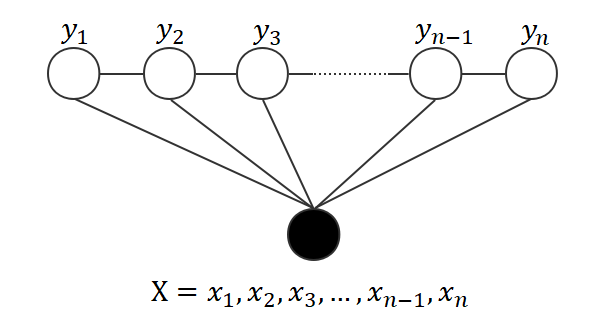
\includegraphics[width=0.9\textwidth]{./figure/线性链条件随机场.jpg}
\caption{线性链条件随机场}
\label{lab:1}
\end{minipage}
\end{figure}

条件随机场实际上是定义在时序数据上的对数线性模型,具有表达长距离依赖性和交叠性特征的能力,能够较好地解决标注偏置等问题。

\section{词向量}
分布式词嵌入是自然语言处理中一组语言建和特征学习技术的总称。将词汇表中的单词或短语映射成预定好维数的实数向。从数学空间映射的角度来看,这个过程是将一个维数等于不同词语数量的空间映射到一个连续的低维向量空间。生成这样映射的方法有神经网络、基于词共现的维数约减等方法。将词语等文本信息通过这样的分布式表现形式作为嵌入,这样的方法已经被证明可以提高自然语言处理任务的效果。

将文本表达成计算机可以理解的形式是自然语言处理任务的第一步。最早最朴素的表示方法是独热表示法(One-hot Representation),即用向量的每一维表示词库中的一个词。例如:

“中国”表示为[1,0,0,0,……,0,0]

“美国”表示为[0,1,0,0,……,0,0]

显然向量的维数是词语的总数,这样的表示方法简单易于理解,但是浪费极大的空间,而且并不能表现出词语与词语之间的关联。将单词表示为较低维度的向量的技术起源于20世纪60年代信息检索向量空间模型的发展。使用奇异值分解减少维度的数量,然后在20世纪80年代后起引入了潜在语义分析(LSA),2000年Bengio等\cite{Bengio}在一些列论文中提出了神经概率语言模型,通过对学习单词的分布式表示来降低上下文中单词表示的高维性。该领域在2010年后逐渐发展真正成为一种热门的方法,一个重要的原因是在那时向量训练的质量和速度方面取得了重要的进展。许多研究组开始在单词嵌入上投入更多经历。2013年,由Tomas Mikolov领导的谷歌团队创造了Word2Vec这样一个单词嵌入工具包,相较于之前的方法,该模型可以更快地训练出向量空间模型。现今大多说新的单词嵌入技术都是基于神经网络架构,而不是传统的n-gram模型和无监督学习。

训练word2vec有两种经典的模式CBOW和Skip-gram模型。

(1)CBOW

CBOW模型训练的方法是通当前词语的上下文词语来预测改词的向量。因而CBOW(Continuous Bag-of-Words)的输入是当前词上下文的词向量,输出就是当前词的词向量。比如下面这句话,“国家主席/习近平/在/进博会/上/宣布/设立/科创板/,并/于/板块/内/进行/注册制/试点/。”我们上下文窗口取值为6的话,特定词为“科创板”,即我们需要求出“科创板”的词向量,前后各有6个词共12个,这12个词是CBOW模型的输入,在最基本的CBOW模型中,采用的是词袋模式,即这12个词的权重一致,并不考虑每个词和目标词的距离。

\begin{figure}[h]
\centering
\begin{minipage}[t]{0.5\textwidth}
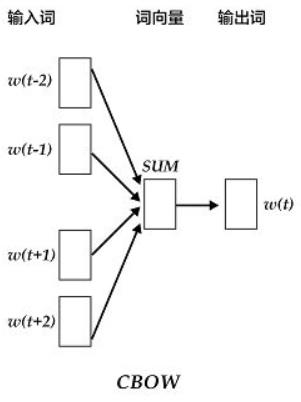
\includegraphics[width=0.9\textwidth]{./figure/CBOW模型.jpg}
\caption{CBOW模型}
\label{lab:1}
\end{minipage}
\end{figure}

CBOW模型的网络结构如图所示,在CBOW模型中输入的是12个词向量,输出的是所有词的softmax概率,损失函数是期望u内联网本特定词对应的softmax概率最大。对应的CBOW模型输入层是12个神经元,输出层的个数和词汇表的总大小一致,有词汇表大小个神经元。隐藏层的神经元个数可以自行设定,对于神经网络的求解通过经典的反向传播算法求解,迭代完所有语料便可以求解出所有词汇表中的词向量。

(2)Skip-gram

\begin{figure}[h]
\centering
\begin{minipage}[t]{0.5\textwidth}
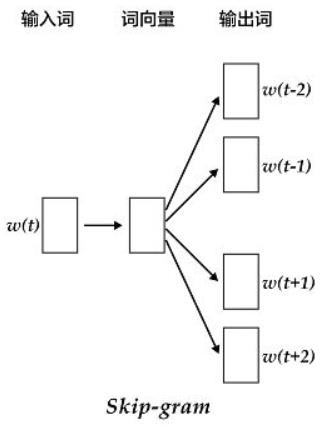
\includegraphics[width=0.9\textwidth]{./figure/Skip-gram模型.jpg}
\caption{Skip-gram模型}
\label{lab:1}
\end{minipage}
\end{figure}

Skip-gram模型与CBOW模型相反,Skip-gram是输入特定的一个词向量,反而输出的上下文的词向量,例如上文的例子的话输出的就是上下文12个词的词向量,同样用反向传播算法,求出概率排前12的softmax该列车对应的神经元对应的词即为所求。

word2vec有许多重要的参数直接决定了训练的效果。上下文窗口决定了给订单词前后包含多少个单词作为上下文单词,在原始的word2vec模型中窗口内各个单词的权重一直,也有一些研究加权词向量的训练方法\cite{myh}来提高词向量的质量。维度也是影响词向量的因素之一,研究表明嵌入词的质量随着维数的增加而提高,但达到某一点后,边际效益将减少\cite{Mikolov}。
在word2vec模型实际运作中,为了解决词汇表太大,训练时间太长的问题,哈会使用霍夫曼树等方法优化训练过程,节省训练的时间。半采样也是实际word2vec训练中常用的优化方法,因为高频词通常提供的信息很少,频率高于设定阈值的单词会被降采样来提高训练的速度和质量。

\section{循环神经网络}

深度学习是基于学习数据表示的更广泛机器学习方法的一种,深度神经网络是深度学习中最重要,应用最广的模型。深度神经网络体系结构已应用与计算机视觉、语音识别、自然语言处理、音频识别、机器翻译、生物信息学、药物设计、医学图像分析等领域。递归神经网络是一类人工神经网络,这类网络善于 预测未来。常用于分析时间序列数据,例如股票价格;在自动驾驶中可以预测汽车的行驶轨迹,避免事故。总的来说这样的网络可以输入文本、句子、语音等,使用到机器翻译、语音识别、语义分析等任务中。

\begin{figure}[h]
\centering
\begin{minipage}[t]{\textwidth}
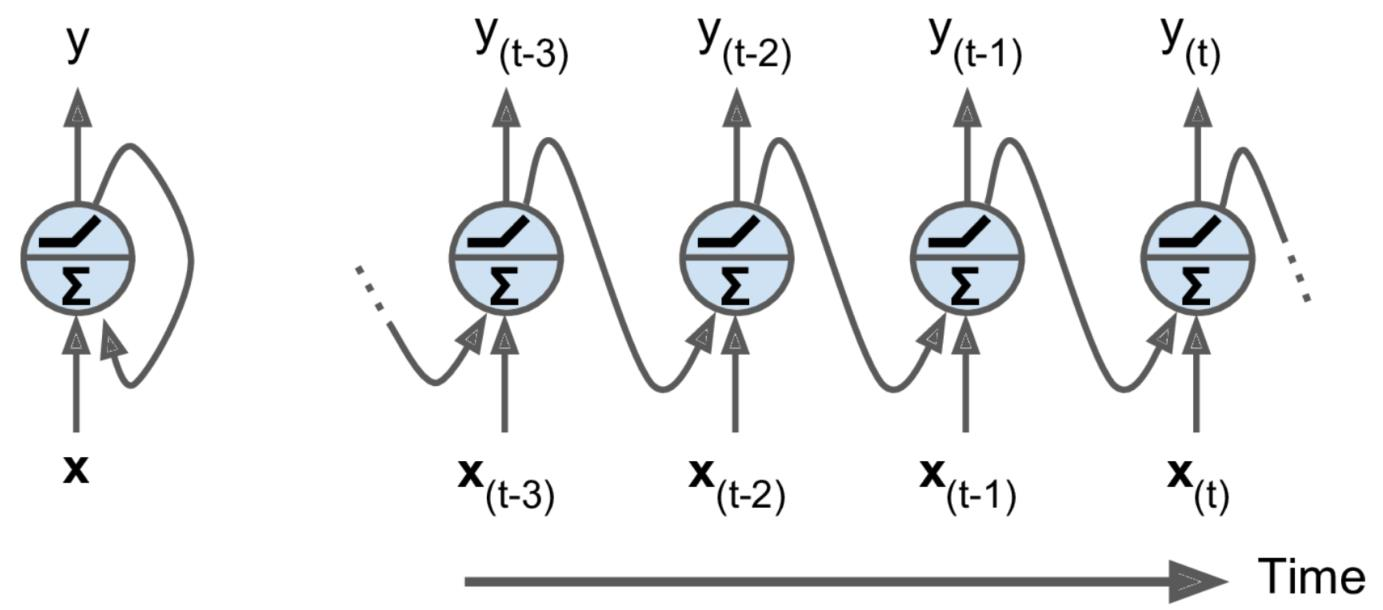
\includegraphics[width=0.9\textwidth,height=5cm]{./figure/simple_rnn.jpg}
\caption{简单的RNN模型}
\label{lab:1}
\end{minipage}
\end{figure}

不同于前馈神经网络,循环神经网络激活方向不仅仅只向一个方向流动。最简单的RNN,只由一个神经元接受输入产生输出,然后将输出发回自身,如图所示。







\section{概率隐语义分析技术}

\section{本章小结}

\chapter{改进的中文字符级特征表示方法}

\section{引言}

\section{相关理论与工作}

\section{面向位置信息的字符向量优化方法}

\section{面向主题信息的字符向量构造方法}

\section{结合位置信息与主题信息的中文字符级特征表示方法}

\section{本章小结}

\chapter{面向复杂命名实体识别的层次深度神经网络模型}

\section{引言}

\section{复杂命名实体概述与相关工作}

\section{层次标签与层次深度神经网络模型构建}

\section{实验结果及分析}

\section{本章小结}

\chapter{中文复杂命名实体识别在企业风险识别中的应用}

\section{引言}

\section{应用背景}

\section{数据爬虫}

\section{文本分类模块}

\section{命名实体识别模块}

\section{企业风险识别}

\chapter{总结与展望}

\section{工作总结}

\section{不足与展望}


\begin{itemize}
\item 第一章,
\item 第二章,

\end{itemize}



\chapter{相关工作}

\lipsum[1]

\chapter{MPTCP速率分配问题分析}

\lipsum[1]

\section{MPTCP速率分配场景}\label{sec:rate}
\lipsum[1]
\subsection{负载均衡}
\lipsum[1]






\chapter{实验验证}
\lipsum[2]

实验硬件设备如图(\ref{img:1})所示。
\begin{figure}[htbp]
\begin{minipage}[t]{0.5\textwidth}
\centering

\includegraphics[width=0.9\textwidth]{./figure/github.jpg}
\caption{实验硬件设备总览}
\label{img:1}
\end{minipage}
\begin{minipage}[t]{0.5\textwidth}
\centering

\includegraphics[width=0.9\textwidth]{./figure/github.jpg}
\caption{实验测量示意图}
\label{img:2}
\end{minipage}
\end{figure}






\chapter{总结与展望}
\lipsum[1]



%%%%%%%%%%%%%%%%%%%%%%%%%%%%%%%%%%%%%%%%%%%%%%%%%%%%%%%%%%%%%%%%%%%%%%%%%%%%%%%
% 致谢,应放在《结论》之后
\begin{acknowledgement}
%thanks
时光荏苒,在南京大学的本科的学习生活即将结束,四年的时间转瞬即逝,这几年的经历必将成为我人生宝贵的财富。在此论文完成之际,谨向这几年来帮助我的老师和同学表达最衷心的感

\end{acknowledgement}

%%%%%%%%%%%%%%%%%%%%%%%%%%%%%%%%%%%%%%%%%%%%%%%%%%%%%%%%%%%%%%%%%%%%%%%%%%%%%%%




% 参考文献。应放在\backmatter之前。
% 推荐使用BibTeX,若不使用BibTeX时注释掉下面一句。
%\nocite{*}
\bibliography{sample}


% 附录,必须放在参考文献后,backmatter前
\appendix
\chapter{MPTCP内核源代码修改}\label{app:1}
\section{函数mptcp\_v4\_subflows()}
\begin{lstlisting}[language=C]
static void mptcp_v4_subflows(struct sock *meta_sk, const struct mptcp_loc4 *loc, struct mptcp_rem4 *rem)
{
   int i;
   int num;
   printk(KERN_INFO "******** Entering mptcp_v4_subflows ********\n");

   initial_my_global_var();
   switch(my_counter)
   {
		case 1 : num = Fir; break;
		case 2 : num = Sec; break;
		case 3 : num = Thi; break;
		default : num = Fir;
	}

	for (i = 1; i < num; i++)
	{
		printk(KERN_INFO "******** in mptcp_v4_subflows i = %d num = %d********\n",i,num);
		mptcp_init4_subsockets(meta_sk, loc, rem);
	}
	printk(KERN_INFO "******** Leaving mptcp_v4_subflows ********\n");
}
\end{lstlisting}

%%%%%%%%%%%%%%%%%%%%%%%%%%%%%%%%%%%%%%%%%%%%%%%%%%%%%%%%%%%%%%%%%%%%%%%%%%%%%%%
% 书籍附件
\backmatter
%%%%%%%%%%%%%%%%%%%%%%%%%%%%%%%%%%%%%%%%%%%%%%%%%%%%%%%%%%%%%%%%%%%%%%%%%%%%%%%
% 作者简历与科研成果页,应放在backmatter之后
\begin{resume}
% 论文作者身份简介,一句话即可。
\begin{authorinfo}
\noindent 韦小宝,男,汉族,1985年11月出生,江苏省扬州人。
\end{authorinfo}
% 论文作者教育经历列表,按日期从近到远排列,不包括将要申请的学位。
\begin{education}
\item[2007年9月 --- 2010年6月] 南京大学计算机科学与技术系 \hfill 硕士
\item[2003年9月 --- 2007年6月] 南京大学计算机科学与技术系 \hfill 本科
\end{education}
% 论文作者在攻读学位期间所发表的文章的列表,按发表日期从近到远排列。
\begin{publications}
\item Xiaobao Wei, Jinnan Chen, ``Voting-on-Grid Clustering for Secure
  Localization in Wireless Sensor Networks,'' in \textsl{Proc. IEEE International
    Conference on Communications (ICC) 2010}, May. 2010.
\item Xiaobao Wei, Shiba Mao, Jinnan Chen, ``Protecting Source Location Privacy
  in Wireless Sensor Networks with Data Aggregation,'' in \textsl{Proc. 6th
    International Conference on Ubiquitous Intelligence and Computing (UIC)
    2009}, Oct. 2009.
\end{publications}
% 论文作者在攻读学位期间参与的科研课题的列表,按照日期从近到远排列。
\begin{projects}
\item 国家自然科学基金面上项目``无线传感器网络在知识获取过程中的若干安全问题研究''
(课题年限~2010年1月 --- 2012年12月),负责位置相关安全问题的研究。
\item 江苏省知识创新工程重要方向项目下属课题``下一代移动通信安全机制研究''
(课题年限~2010年1月 --- 2010年12月),负责LTE/SAE认证相关的安全问题研究。
\end{projects}
\end{resume}

%%%%%%%%%%%%%%%%%%%%%%%%%%%%%%%%%%%%%%%%%%%%%%%%%%%%%%%%%%%%%%%%%%%%%%%%%%%%%%%
% 生成《学位论文出版授权书》页面,应放在最后一页
%\makelicense

%%%%%%%%%%%%%%%%%%%%%%%%%%%%%%%%%%%%%%%%%%%%%%%%%%%%%%%%%%%%%%%%%%%%%%%%%%%%%%%
\end{document}
